This supplement follows the original Materials and Methods topic sequence, then Figures S1--S15 and Tables S1--S2. It reports only outcomes supported by the saved independent calculations. Detailed processing settings, input inventories, assumptions and validation are collected after this supplement.

\section*{Materials and Methods}
\section{Building the Campi Flegrei high-resolution earthquake catalog}
\paragraph{Data.} The independently retrieved station intervals and station inventory provide partial counterparts to Figures S1 and S2. They do not establish complete network coverage over the study period.
\paragraph{Phase picking.} Inference with released trained weights produced 3,637 merged picks (560 P and 3,077 S). The training examples and exact benchmark windows in Figures S3 and S4 were not reproduced. Inference on other windows is supporting evidence only.
\paragraph{Phase association.} GaMMA associated 63 picks into nine provisional events. These results are insufficient to replace the paper's later location products.
\paragraph{Initial earthquake location.} Three events passed the stated geometry screen, but no scientific VELEST inversion was run. Figure S6 and Table S1 therefore have no independent counterpart. The current external routine catalog is contextual evidence for S5, not a replacement for independent locations.
\paragraph{Earthquake relocation.} Neither TomoDD relocation nor regional HypoDD SVD uncertainty estimation has been executed. Figures S7 and S9--S13 retain their unreproduced status.
\paragraph{Local magnitude.} Of 140 measured channel amplitudes, 23 passed the 5 dB SNR threshold, but no event pair supplied a qualifying magnitude-difference equation. There are no calibrated magnitudes, completeness estimate or b-value for Figure S8.
\paragraph{Focal mechanism estimation.} SKHASH and gCAP inversions were not run. No independent mechanism is available for Figure 4.

\section{Validation of earthquake locations}
\paragraph{Ring-shaped structures with confined depth distributions.} The provisional associations do not establish a ring structure. Internal travel-time consistency is preserved in the documentation, but does not substitute for the regional uncertainty or common-receiver tests in Figures S7 and S12.
\paragraph{Depth of earthquakes in the central region.} No associated CPOZ P arrival exists in the processed sample. The specified CPOZ waveform gathers and manual checks on apparently deep central events remain unperformed. No conclusion about a lower depth limit follows from their absence.

\section{Template Matching to Detect Hybrid Events}
The search covered 24.298 hours of available common CAAM/COLB intervals and returned four unconfirmed candidates. It did not produce independently confirmed families for Figure S14.
\paragraph{Depth.} No independent hybrid-event location set is available for Table S2.
\paragraph{Frequency index.} Frequency indices were calculated for the available template and candidate windows. Figure S15C displays the corresponding third written-method template. The first two templates are different examples from the published S15A/B panels and are not inserted in their place.
\paragraph{Relative magnitude.} Cluster-relative magnitudes were not assigned because cluster membership has not been established.
\paragraph{Temporal evolution of the hybrid events.} The limited exposure and unconfirmed detections do not support a three-year cluster history.
\paragraph{Further search for HB/LP events.} Catalog-wide frequency-index and coda-contamination review remains incomplete.

\clearpage
\section*{Supplementary figures}
\setcounter{figure}{0}
\begin{figure}[H]
\centering
\par\smallskip\textbf{Panel S1; current provisional independent calculation: partially reproduced}\par
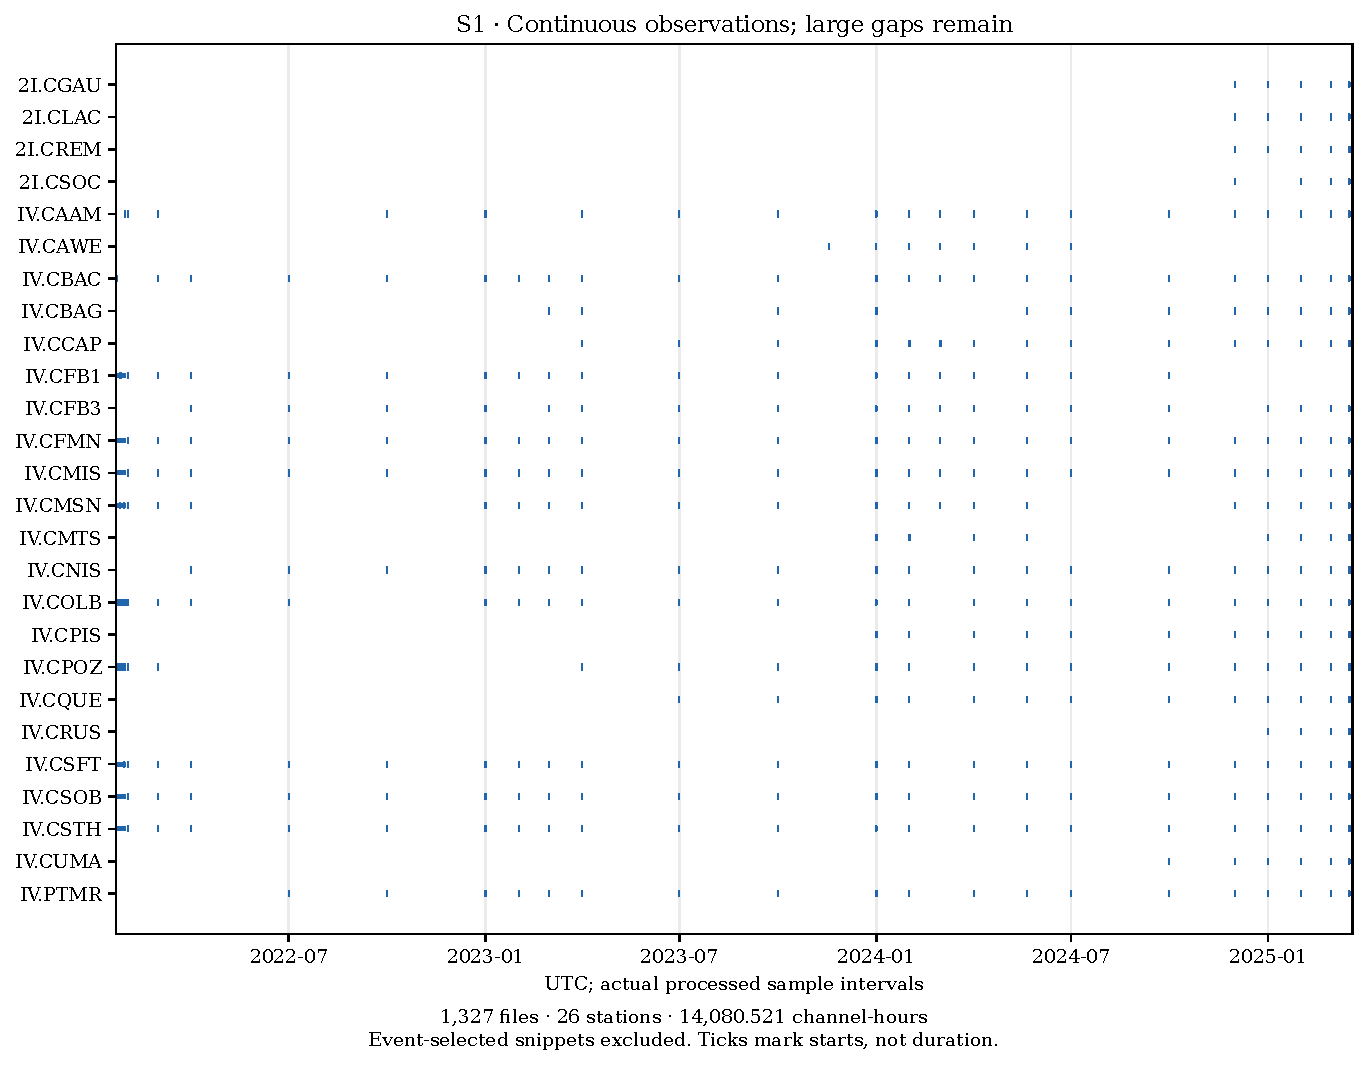
\includegraphics[width=.94\linewidth,height=0.620\textheight,keepaspectratio]{figures/coverage_availability_extension.pdf}
\caption{Recorded station availability. 1,327 eligible continuous files, 14,080.521 processed channel-hours, 26 stations. Actual merged intervals only; ticks identify starts, not duration. Failed and pending requests and event-selected snippets are excluded. Large temporal/network gaps remain.}
\label{publication:S1}
\end{figure}

\begin{figure}[H]
\centering
\par\smallskip\textbf{Panel S2: partially reproduced}\par
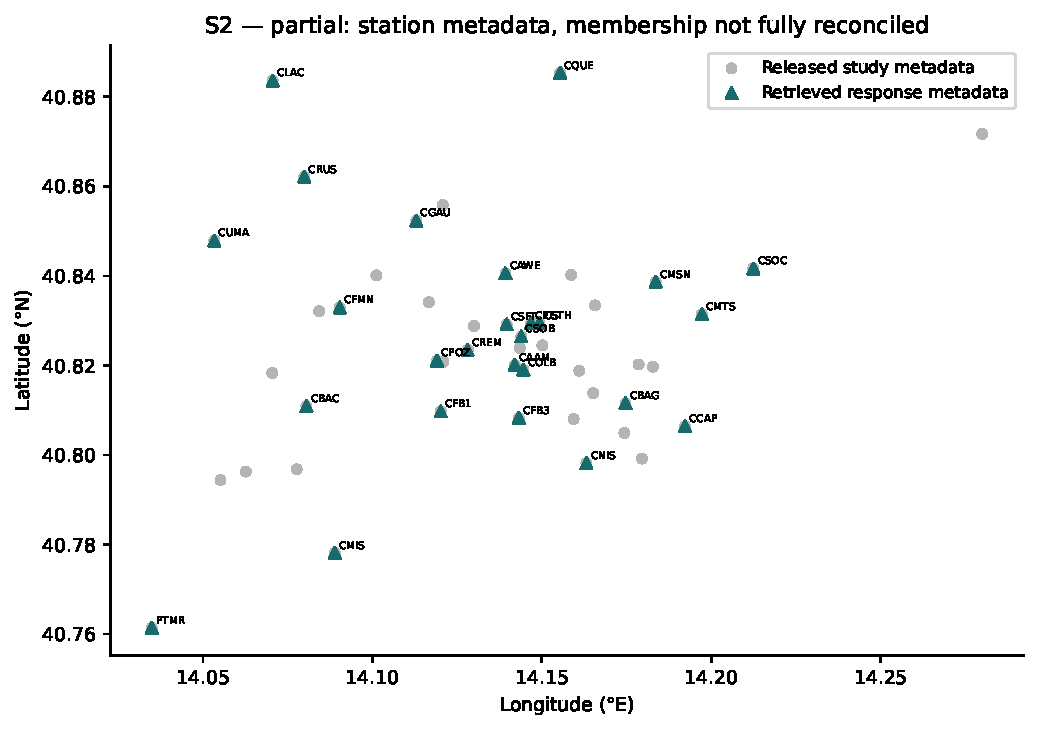
\includegraphics[width=.94\linewidth,height=.66\textheight,keepaspectratio]{figures/stations_partial.pdf}
\caption{Station locations. Partial: released station coordinates and retrieved IV/2I response metadata. Exact membership of the original 48 instruments, station epochs and the basemap are not fully reconciled.}
\label{publication:S2}
\end{figure}

\begin{figure}[H]
\centering
\missingresult{All panels/views}{Panels A--D require the specified training traces, annotations and augmentation examples. These were not reconstructed; downstream use of trained weights is not retraining.}
\caption{Training examples. Noise, single-event and overlapping-event training examples are not reproduced.}
\label{publication:S3}
\end{figure}

\paragraph{Figure S4 --- not reproduced.} Panels A and B were not generated for the exact CSOB swarm and CMIS noise examples. Other unlabeled inference comparisons remain diagnostics.

\setcounter{figure}{4}
\begin{figure}[H]
\centering
\par\smallskip\textbf{Panel S5, all views: partially reproduced}\par
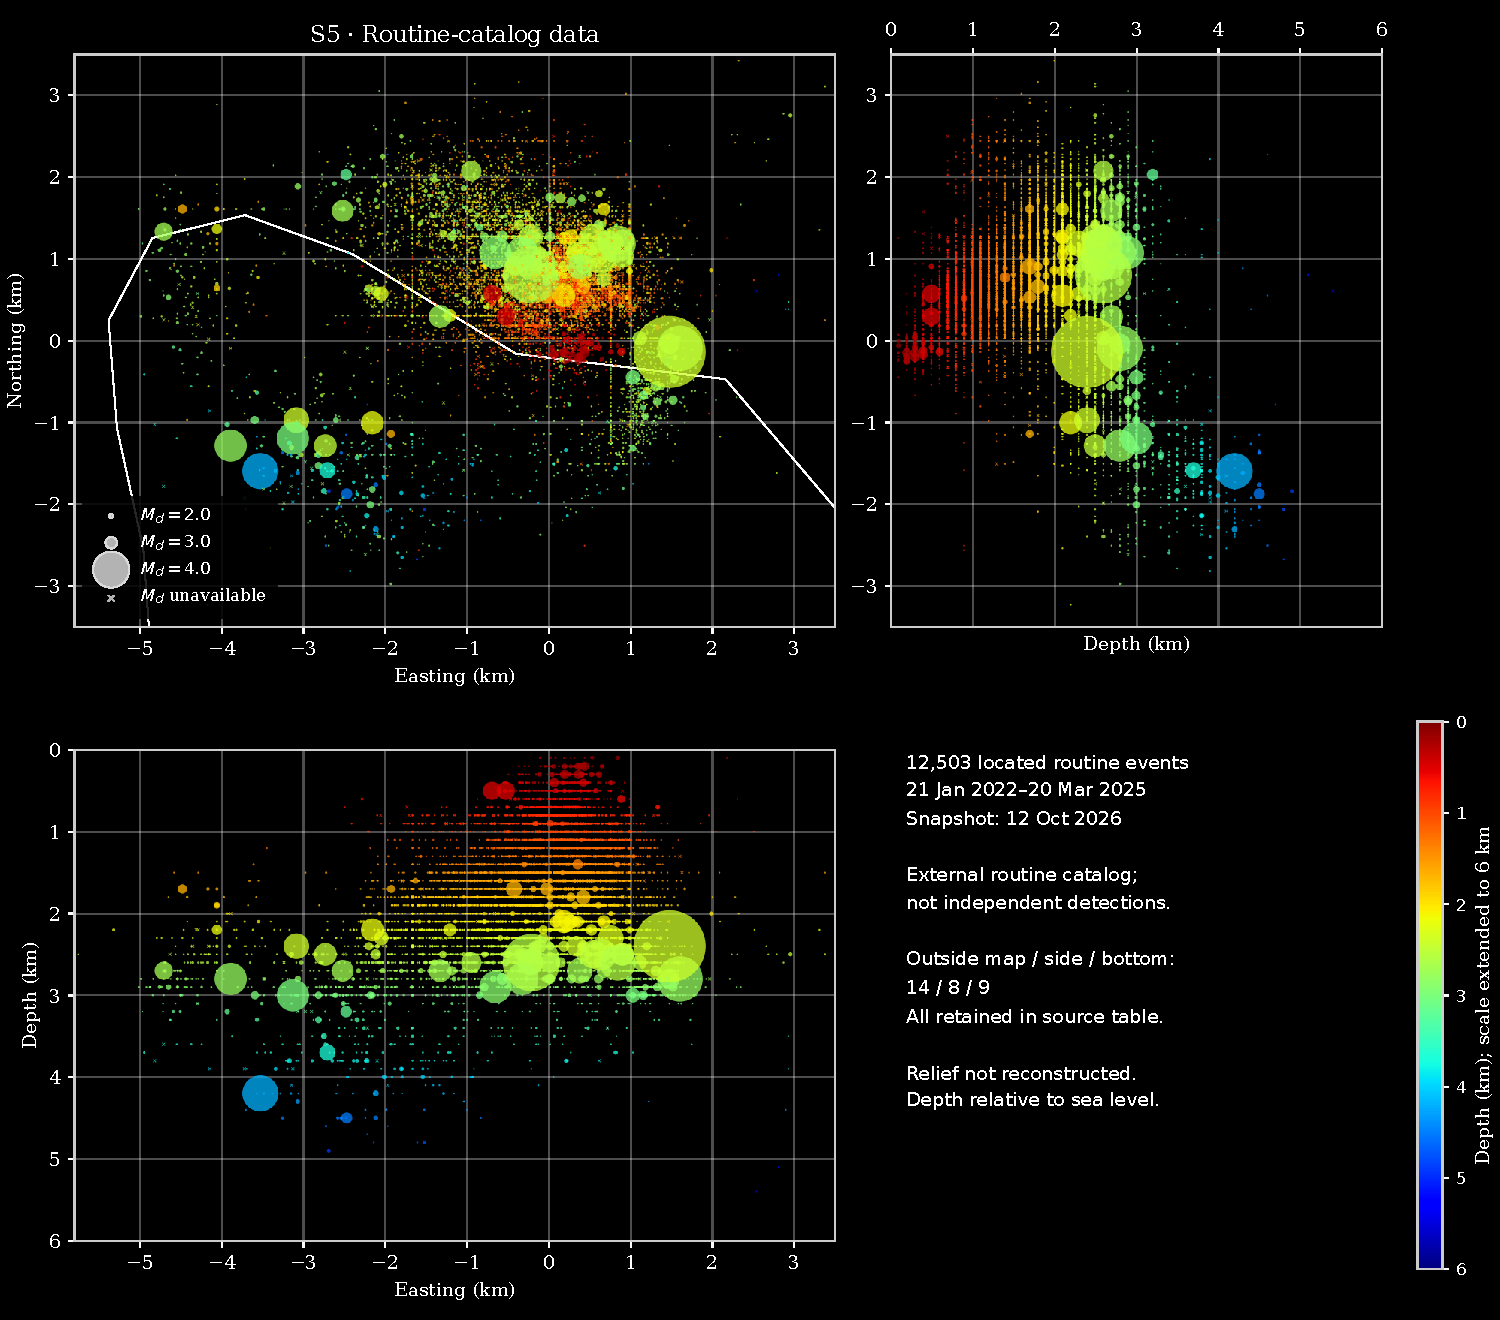
\includegraphics[width=.94\linewidth,height=.66\textheight,keepaspectratio]{figures/figure_S5_routine.pdf}
\caption{Routine-catalog locations. External routine-catalog data, independently selected and plotted: 12,503 located events, 21 January 2022--20 March 2025. This is 420 more than the published historical snapshot. No author-derived catalog is used to adjust that difference; these are not independent detections. Depth colors run red to blue on a dark background; the color scale extends to 6 km to include the observed range. Circle area includes an exponential Md term and a small visibility offset, an explicit display assumption; crosses indicate missing Md. Published pixels are not plotting inputs. The public source reports depths in 0.1 km steps; the resulting bands are not jittered or smoothed.}
\label{publication:S5}
\end{figure}

\setcounter{figure}{5}
\begin{figure}[H]
\centering
\par\smallskip\textbf{Panel S6; provisional numerical counterpart: partially reproduced}\par
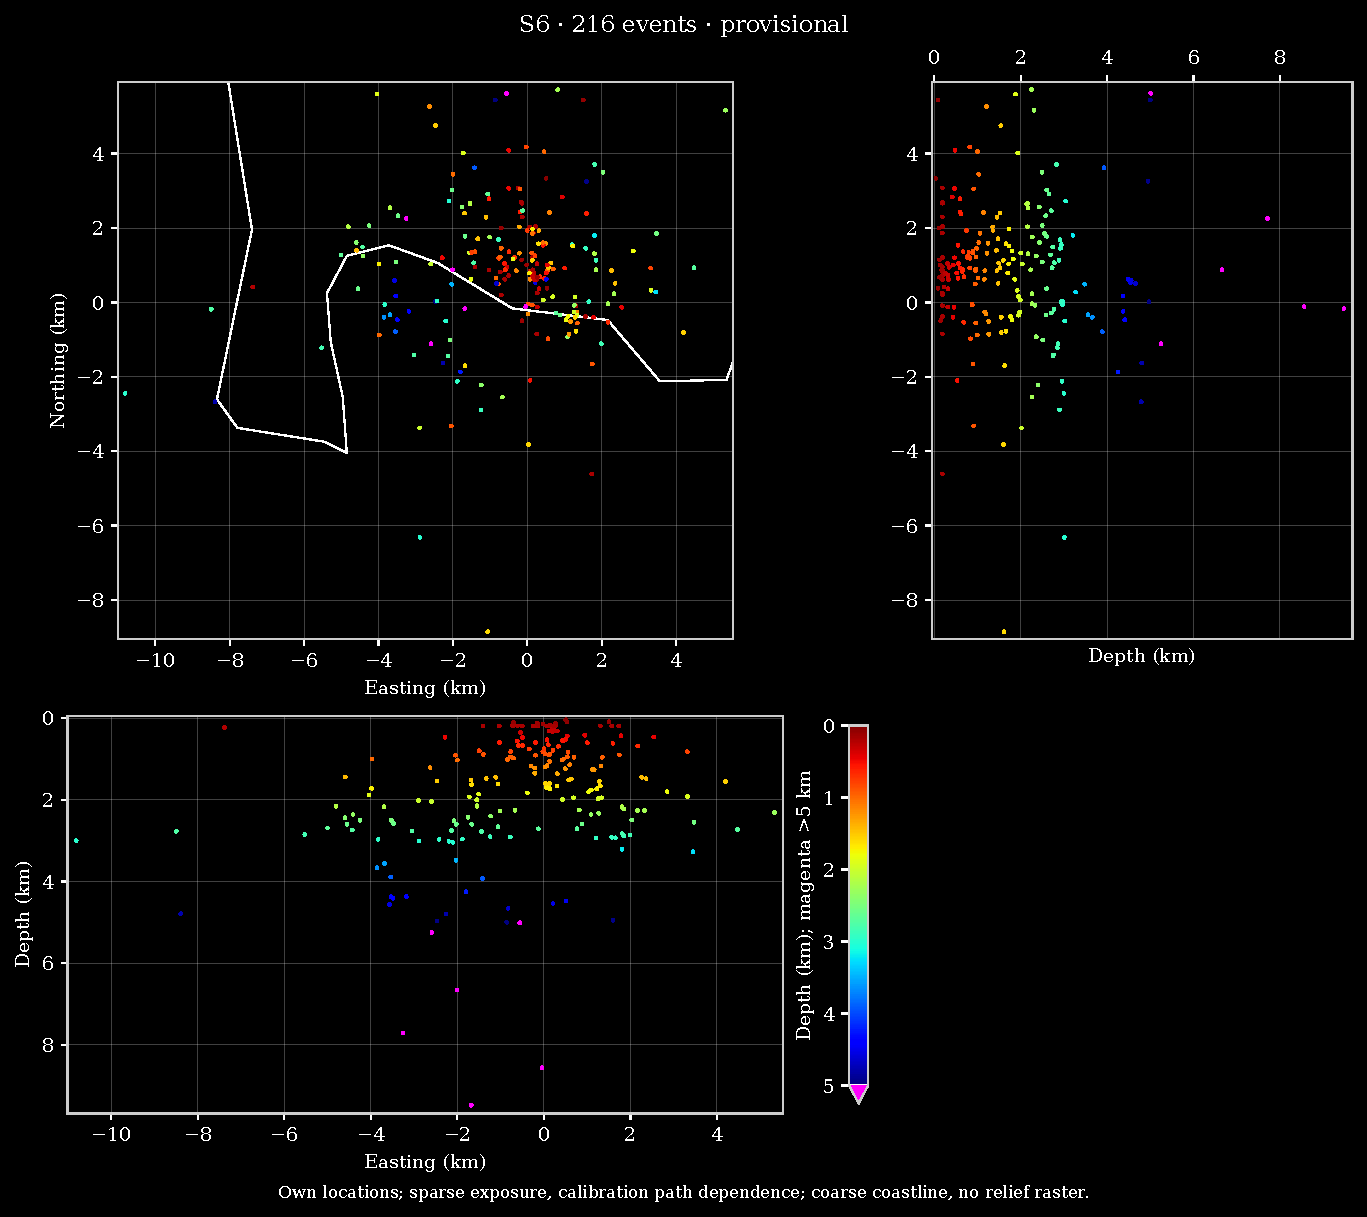
\includegraphics[width=.94\linewidth,height=0.310\textheight,keepaspectratio]{figures/figure_S6_provisional.pdf}
\par\smallskip\textbf{Panel Latest extended cohort: independently rerun, provisional: partially reproduced}\par
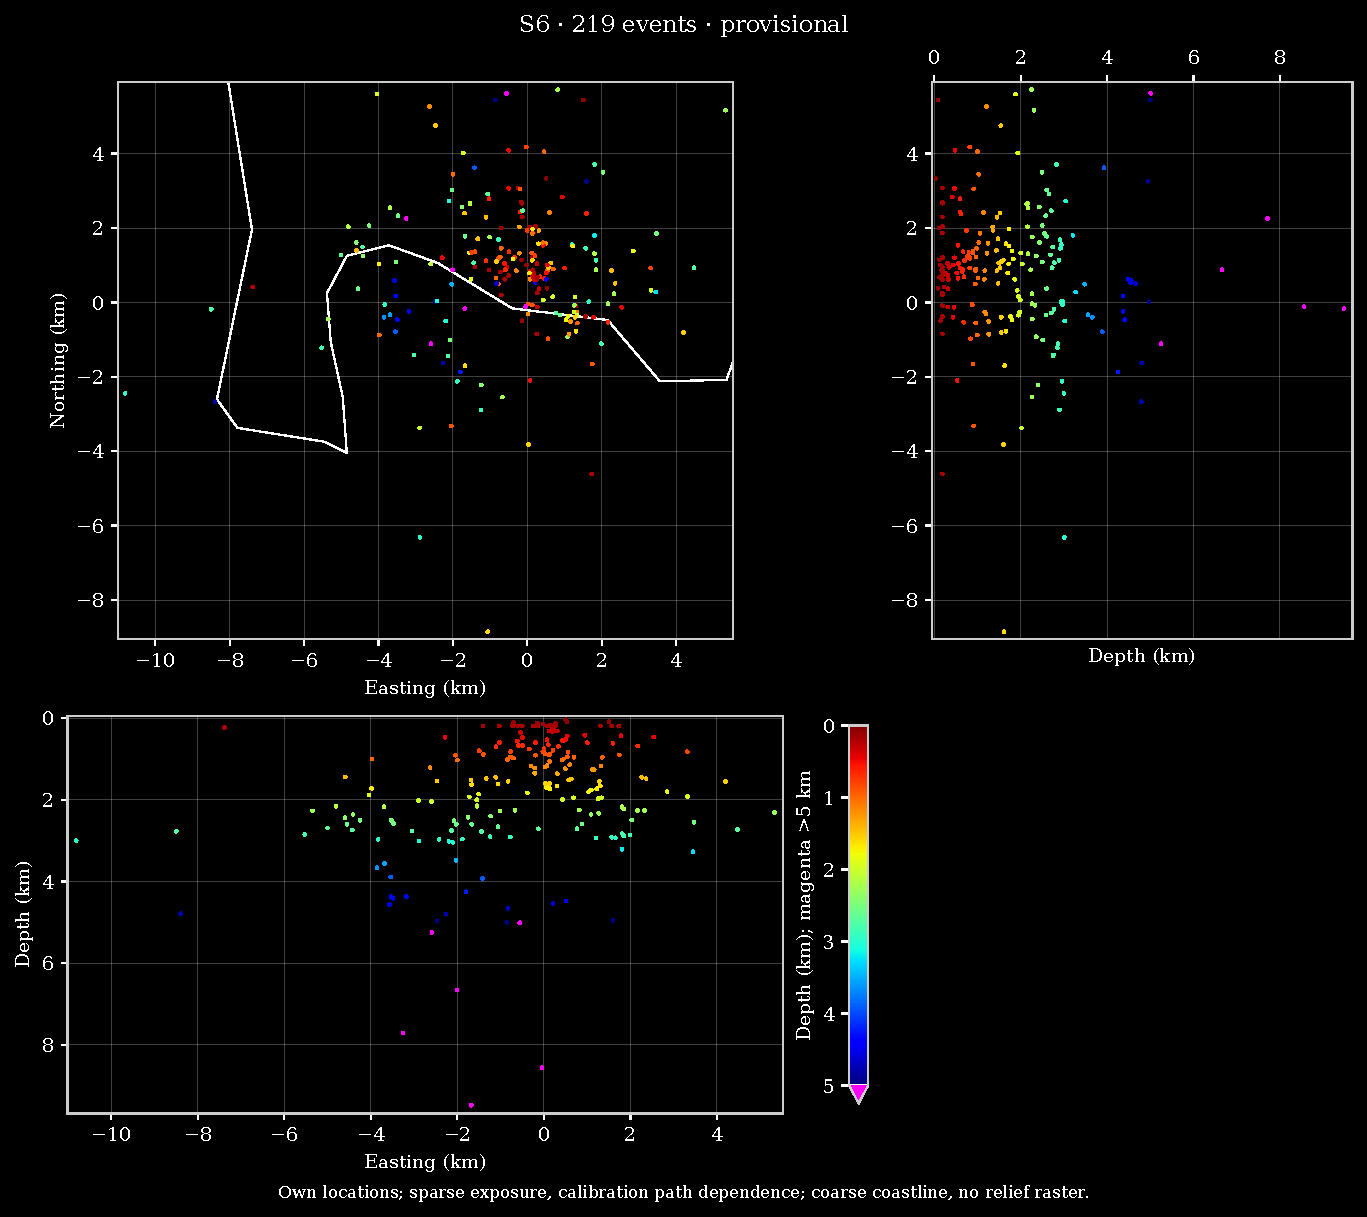
\includegraphics[width=.94\linewidth,height=0.310\textheight,keepaspectratio]{figures/figure_S6_extension.pdf}
\caption{Initial VELEST locations. 216 independently fitted VELEST events pass the numerical pick/RMS/gap filters. Physical layer ordering and the final small-update gate pass; stagnation, held-out prediction, regional and precision-path stability prevent acceptance. These are plotted as provisional results. Provisional independent observations and processing; sparse coverage, unreviewed phases, calibration path sensitivity. Not established fault geometry or exact reproduction. The additional extended-cohort view uses separately numbered, independently rerun results. Magnitudes and SVD uncertainties were not inherited by integer event ID.}
\label{publication:S6}
\end{figure}

\setcounter{figure}{6}
\begin{figure}[H]
\centering
\par\smallskip\textbf{Panel S7; current provisional independent calculation: partially reproduced}\par
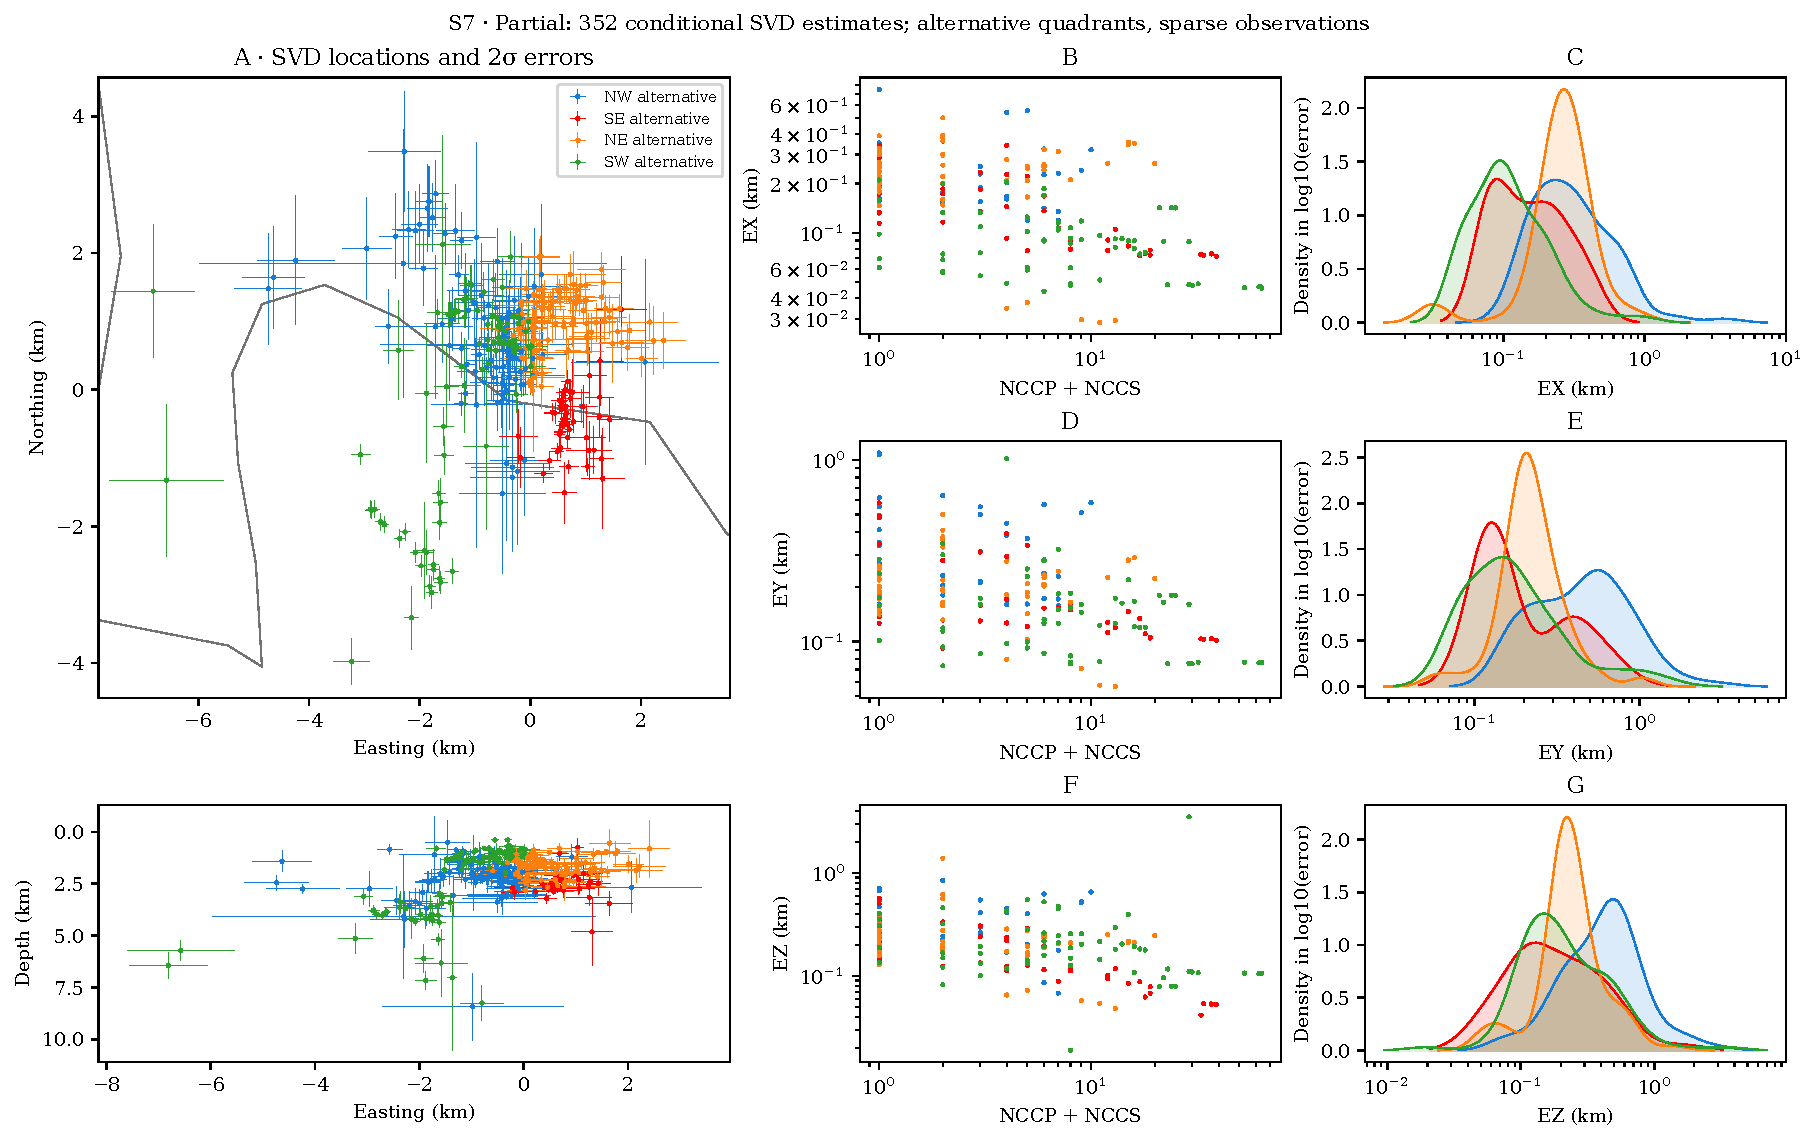
\includegraphics[width=.94\linewidth,height=0.620\textheight,keepaspectratio]{figures/figure_S7_eida_followup.pdf}
\caption{Location uncertainties. 352 conditional HypoDD SVD estimates in four explicitly alternative geographic subsets. Maximum vertical 2-sigma error 3.499 km. Regional samples are capped at the written 174/165/175/166 events with disclosed seed 42; membership is saved. Model and phase-identification biases are not included; zero correlation counts omitted only from logarithmic axes. Partial/provisional: sparse observations, alternative association profile, unreviewed phases and unresolved model/location accuracy. Numerical generation is not agreement with the publication.}
\label{publication:S7}
\end{figure}

\begin{figure}[H]
\centering
\missingresult{All panels/views}{Panels A and B require qualifying relative-amplitude equations and calibrated magnitudes. Zero qualifying equations were obtained; completeness and b-value were not estimated.}
\caption{Magnitude calibration and frequency distribution. Local-versus-duration magnitude comparison and magnitude-frequency distribution are not reproduced.}
\label{publication:S8}
\end{figure}

\begin{figure}[H]
\centering
\missingresult{All panels/views}{All three views require independently relocated events and cross-correlation observation counts for the published quality filter. These outputs are absent.}
\caption{Best-located earthquake subset. The filtered map and cross sections are not reproduced.}
\label{publication:S9}
\end{figure}

\begin{figure}[H]
\centering
\missingresult{All panels/views}{The four annual groups for 2022--2025 require the independent multiyear relocated catalog. The available sample does not support them.}
\caption{Seismicity by year. All four annual groups are not reproduced.}
\label{publication:S10}
\end{figure}

\setcounter{figure}{10}
\begin{figure}[H]
\centering
\par\smallskip\textbf{Panel S11; latest provisional numerical counterpart: partially reproduced}\par
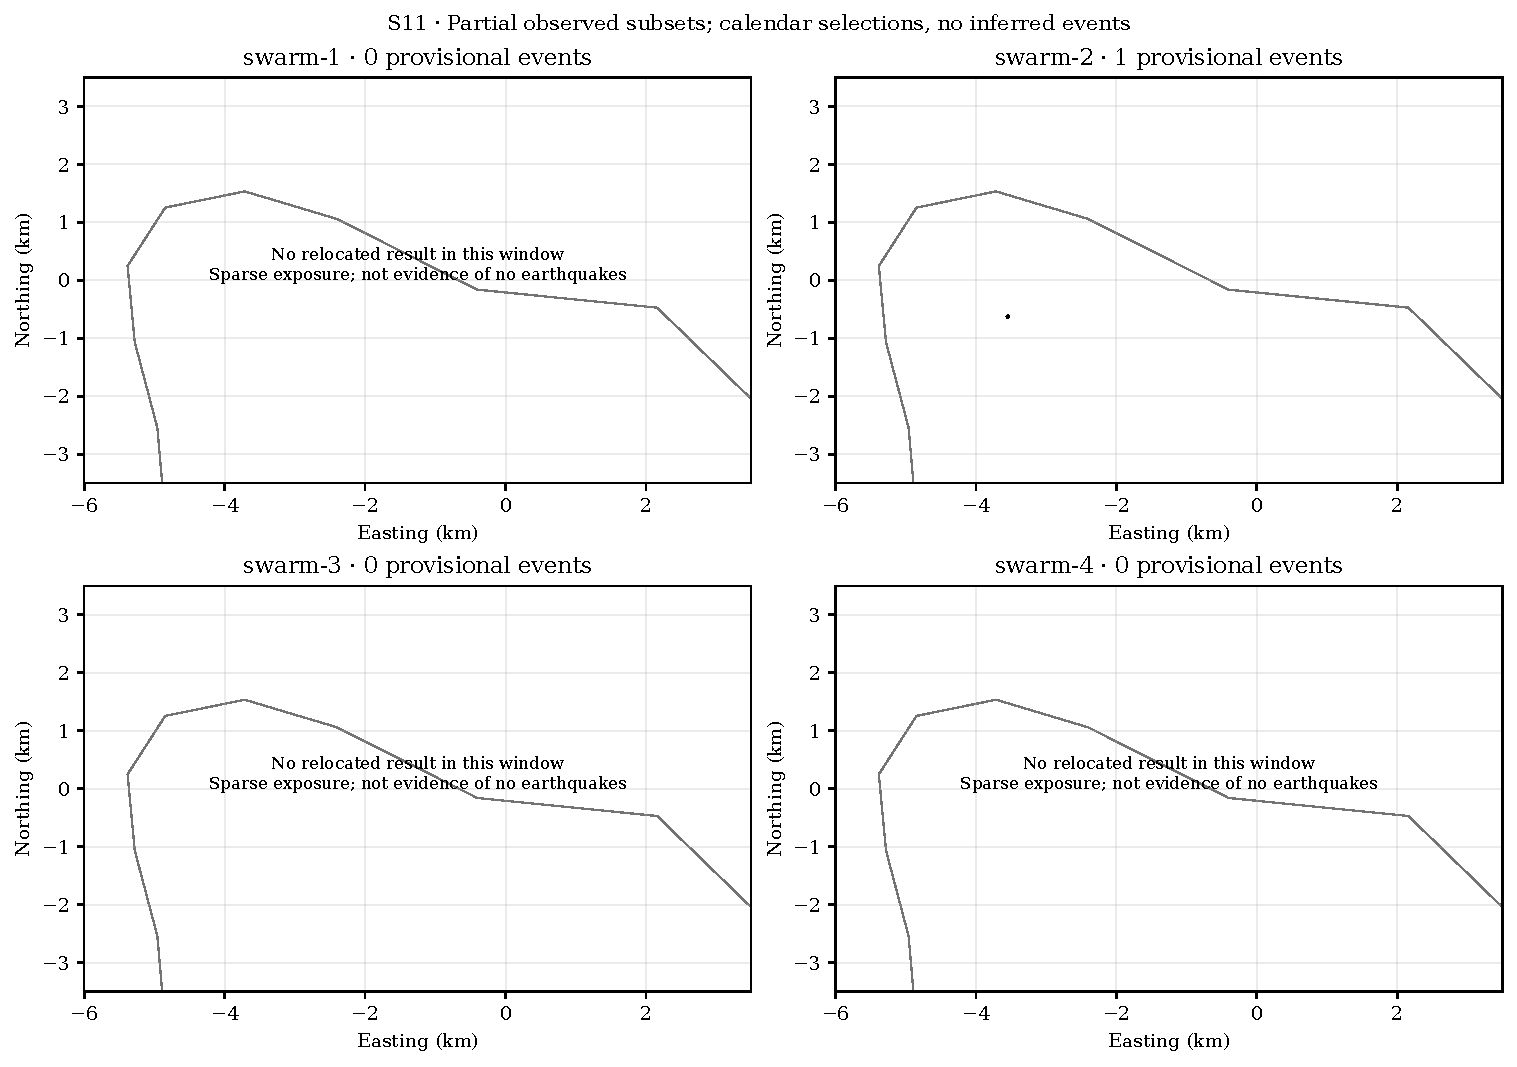
\includegraphics[width=.94\linewidth,height=0.620\textheight,keepaspectratio]{figures/figure_S11_local_followup.pdf}
\par\small S11/swarm-1, swarm-3 and swarm-4 have no surviving independently relocated events in their written calendar windows; sparse exposure, not evidence that no earthquakes occurred.
\caption{Four major swarms. Written calendar windows, inclusive end days. Only swarm 2 contains one retained independent event; the other windows have no qualifying result. Empty selections are not evidence that earthquakes did not occur. Sparse observations, unreviewed phases and unresolved calibration sensitivity; partial numerical counterpart, not accepted structural reproduction.}
\label{publication:S11}
\end{figure}

\begin{figure}[H]
\centering
\missingresult{All panels/views}{Panels A--H require relocated sector selections and independently associated CPOZ P arrivals. The current associations contain zero CPOZ P arrivals.}
\caption{Ring sectors and CPOZ common-receiver gathers. Sector views and six arrival-aligned waveform gathers are not reproduced.}
\label{publication:S12}
\end{figure}

\paragraph{Figure S13 --- not reproduced.} Panels A and B require reliable independent relocated coordinates and an appropriately sourced basemap. The relocated catalog does not exist.

\begin{figure}[H]
\centering
\missingresult{All panels/views}{The three clusters and unclustered group require a multiyear scan, confirmed events, frequency indices and cluster-relative magnitudes. Four current candidates are unconfirmed.}
\caption{Hybrid-event clusters. Cluster histories and annotated waveform collections are not reproduced.}
\label{publication:S14}
\end{figure}

\setcounter{figure}{14}
\begin{figure}[H]
\centering
\par\smallskip\textbf{Panel S15A analogue: different documented E1 event: partially reproduced}\par
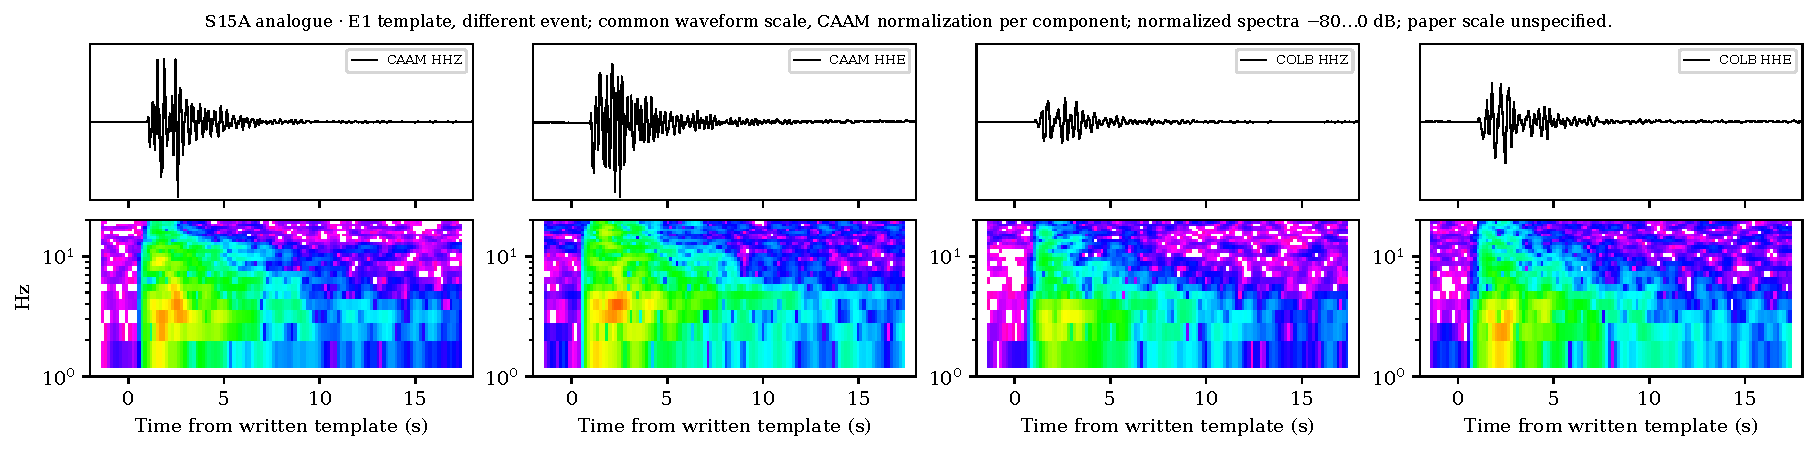
\includegraphics[width=.94\linewidth,height=0.207\textheight,keepaspectratio]{figures/hybrid_E1.pdf}
\par\smallskip\textbf{Panel S15B analogue: different documented E2 event: partially reproduced}\par
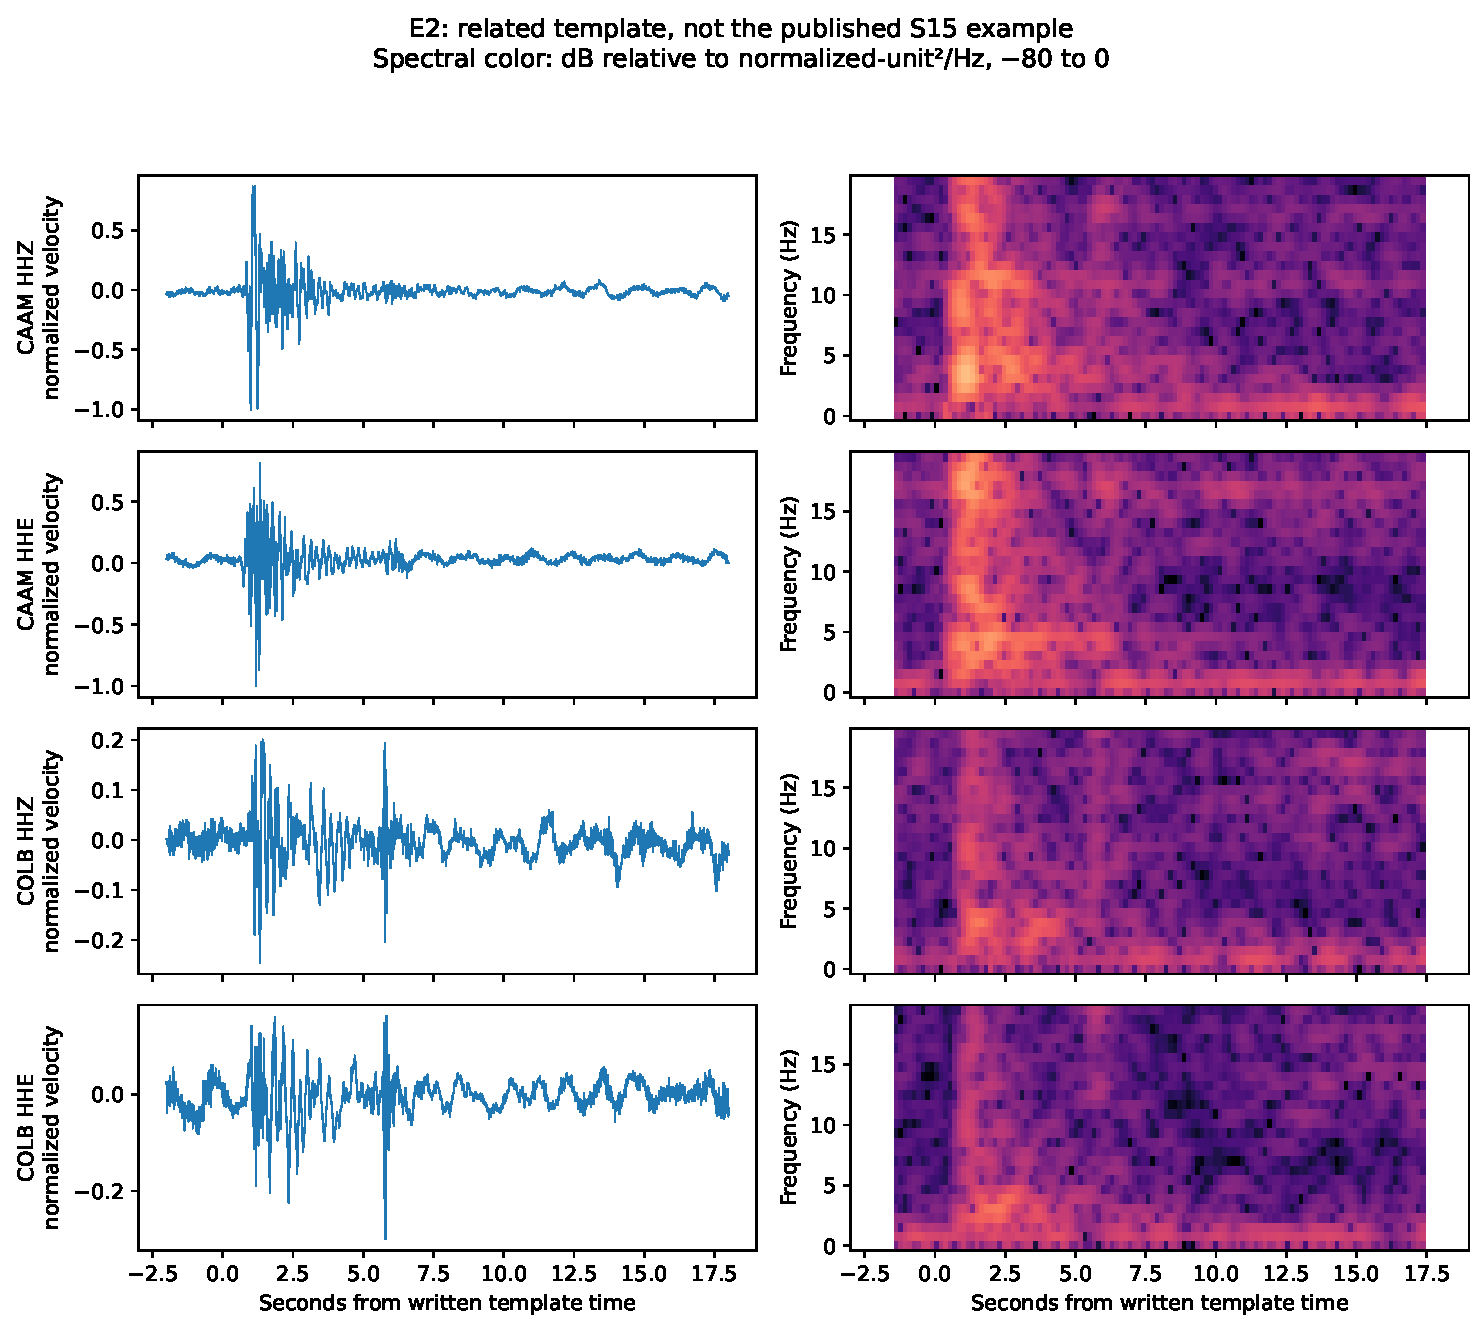
\includegraphics[width=.94\linewidth,height=0.207\textheight,keepaspectratio]{figures/hybrid_E2.pdf}
\par\smallskip\textbf{Panel S15C: documented E3 event: partially reproduced}\par
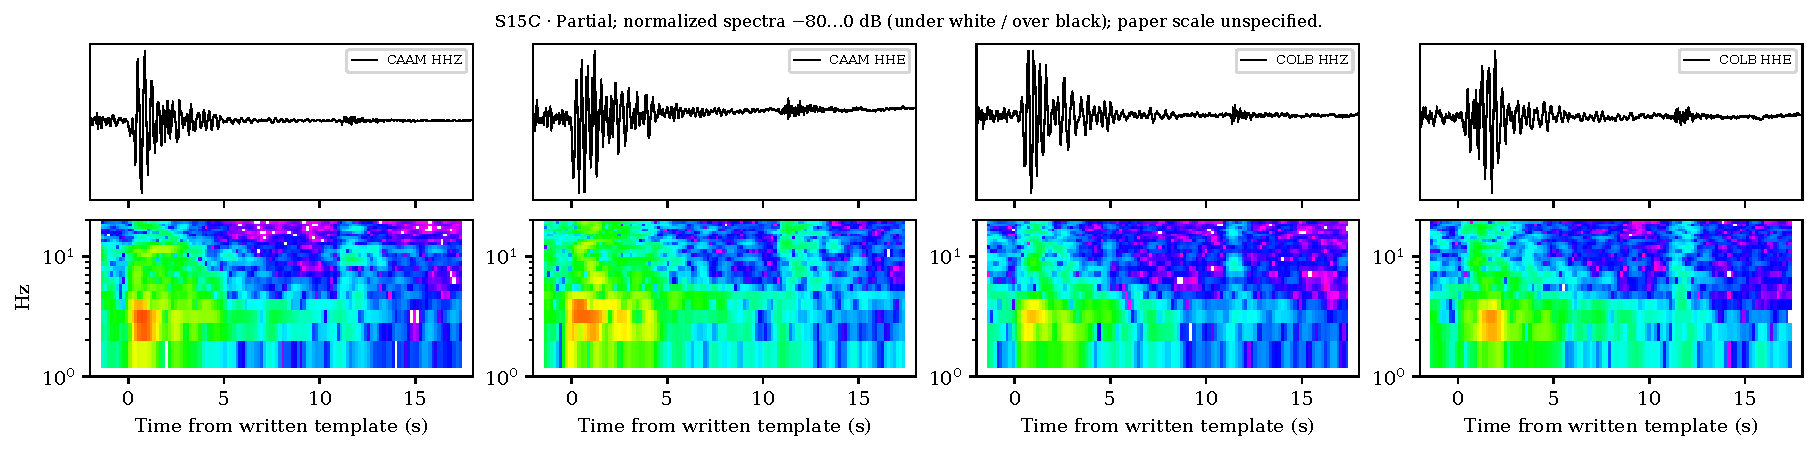
\includegraphics[width=.94\linewidth,height=0.207\textheight,keepaspectratio]{figures/hybrid_E3.pdf}
\par\small S15D: no retained independently relocated event with depth <0.6 km south of 40.83 N in this cohort, hence no suitable west-Accademia extremely-shallow example. Incorrectly labeled examples are not substituted.
\caption{Hybrid and shallow-event waveforms. Partial numerical waveform/spectral counterparts. A/B analogues use the written-method E1/E2 family templates, which are different events from the published A/B examples. They are explicitly not exact event reproduction. C uses E3. All are processed original CAAM/COLB observations; normalization and spectral settings are disclosed. No author waveform or spectral array is used.}
\label{publication:S15}
\end{figure}


\section*{Supplementary tables}
\paragraph{Table S1: fitted one-dimensional velocity model --- not reproduced.}
No independently fitted VELEST model exists. The author's tabulated fitted velocities are not copied into this result.
\paragraph{Table S2: hybrid events in the relocated catalog --- not reproduced.}
No independently relocated hybrid-event sample exists. The author's event parameters are not substituted.

\section*{Supplementary data products}
Independent counterparts of the final catalog (Data S1), associated phases of that final catalog (Data S2), focal mechanisms (Data S3), and the relocated interactive view (Interactive Plot S1) are not complete. The saved provisional products retain their existing labels. References and the complete provenance record follow in the reproduction documentation.
